\documentclass{article}
\usepackage{tikz}
\usepackage{pgf}
\usetikzlibrary{arrows,shapes,positioning,shadows,trees}

\tikzset{
  basic/.style  = {draw, text width=2cm, drop shadow, font=\sffamily, rectangle},
  level 1/.style = {basic, rounded corners=6pt, thin,align=center, fill=green!60,
                   text width=8em}
}

\begin{document}

\section{Mesh, Grids and Coordinates (down-up)}
\noindent
\subsection{Coordinates}
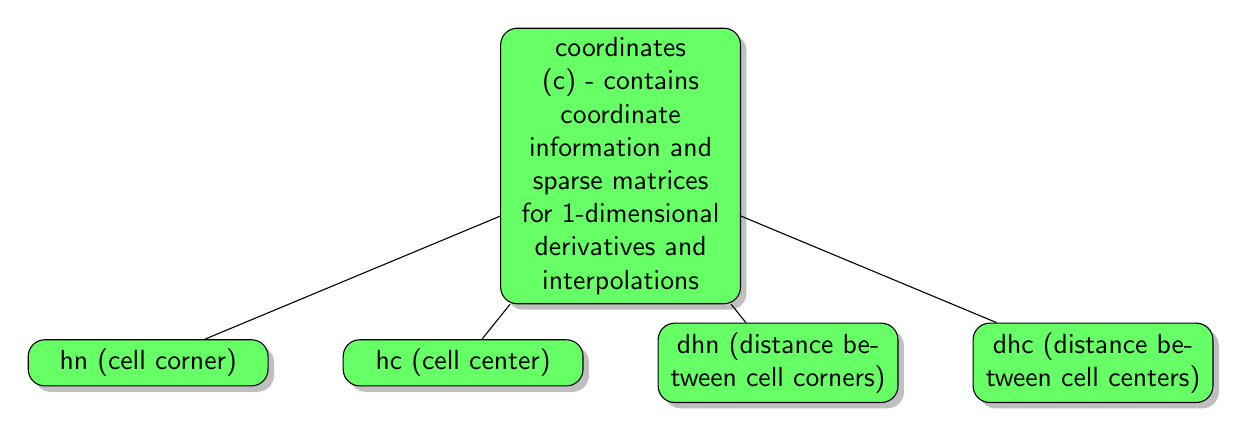
\begin{tikzpicture}[level distance=25mm,level/.style={sibling distance=40mm}]
\node[level 1] {coordinates (c) - contains coordinate information and sparse matrices for 1-dimensional derivatives and interpolations}
		child { node[level 1] (c1) {hn (cell corner)} }
		child { node[level 1] (c1) {hc (cell center)} }
		child { node[level 1] (c1) {dhn (distance between cell corners)} }
		child { node[level 1] (c1) {dhc (distance between cell centers)} };
\end{tikzpicture}
\subsection{Grids}
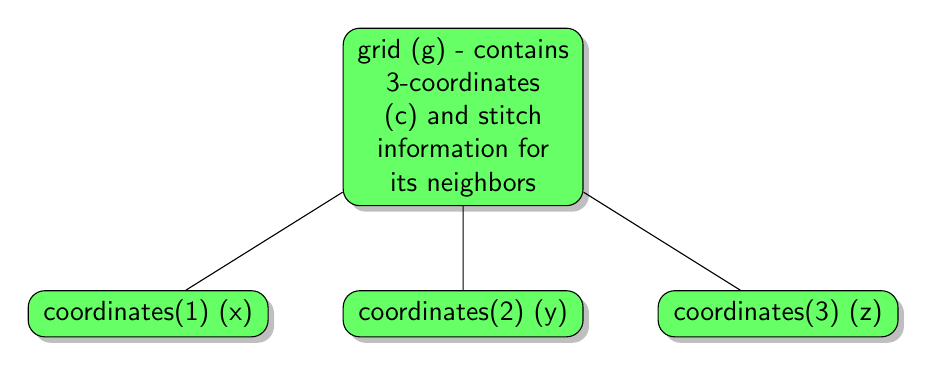
\begin{tikzpicture}[level distance=25mm,level/.style={sibling distance=40mm}]
\node[level 1] {grid (g) - contains 3-coordinates (c) and stitch information for its neighbors}
		child { node[level 1] (c1) {coordinates(1) (x)} }
		child { node[level 1] (c1) {coordinates(2) (y)} }
		child { node[level 1] (c1) {coordinates(3) (z)} };
\end{tikzpicture}
\subsection{Mesh}
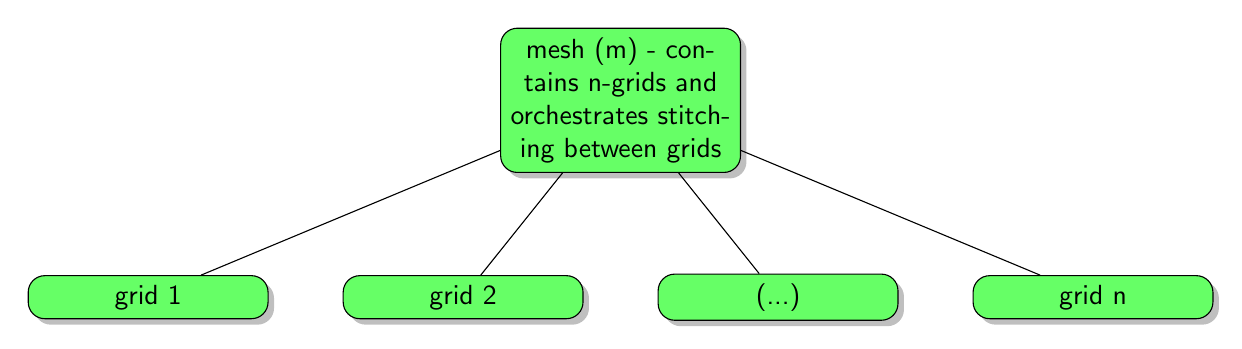
\begin{tikzpicture}[level distance=25mm,level/.style={sibling distance=40mm}]
\node[level 1] {mesh (m) - contains n-grids and orchestrates stitching between grids}
		child { node[level 1] (c1) {grid 1} }
		child { node[level 1] (c1) {grid 2} }
		child { node[level 1] (c1) {(...)} }
		child { node[level 1] (c1) {grid n} };
\end{tikzpicture}


\section{Real field, Scalar and Vector Fields (down-up)}
\subsection{Real-field}
\noindent
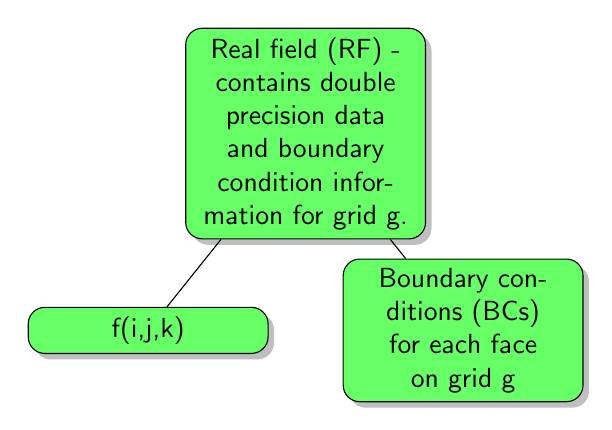
\begin{tikzpicture}[level distance=25mm,level/.style={sibling distance=40mm}]
\node[level 1] {Real field (RF) - contains double precision data and boundary condition information for grid g.}
		child { node[level 1] (c1) {f(i,j,k)} }
		child { node[level 1] (c1) {Boundary conditions (BCs) for each face on grid g} };
\end{tikzpicture}
\subsection{Scalar field}
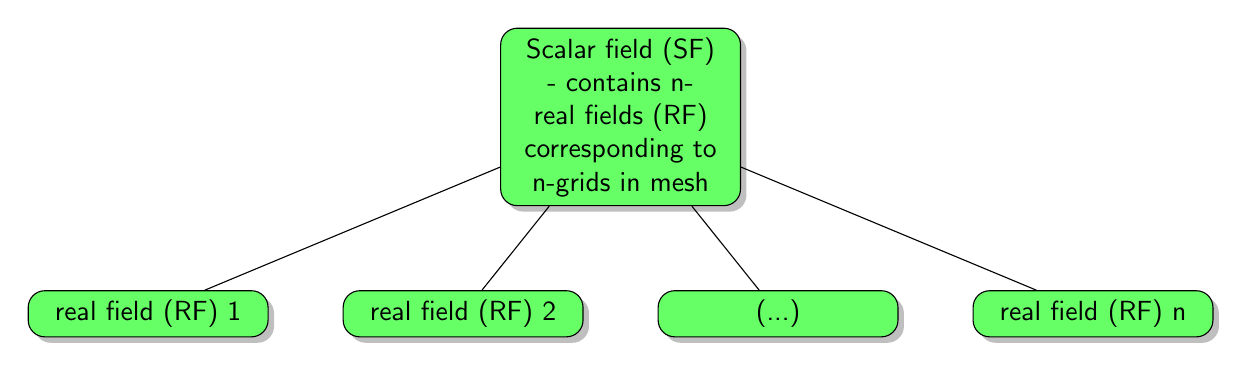
\begin{tikzpicture}[level distance=25mm,level/.style={sibling distance=40mm}]
\node[level 1] {Scalar field (SF) - contains n-real fields (RF) corresponding to n-grids in mesh}
		child { node[level 1] (c1) {real field (RF) 1} }
		child { node[level 1] (c1) {real field (RF) 2} }
		child { node[level 1] (c1) {(...)} }
		child { node[level 1] (c1) {real field (RF) n} };
\end{tikzpicture}
\subsection{Vector field}
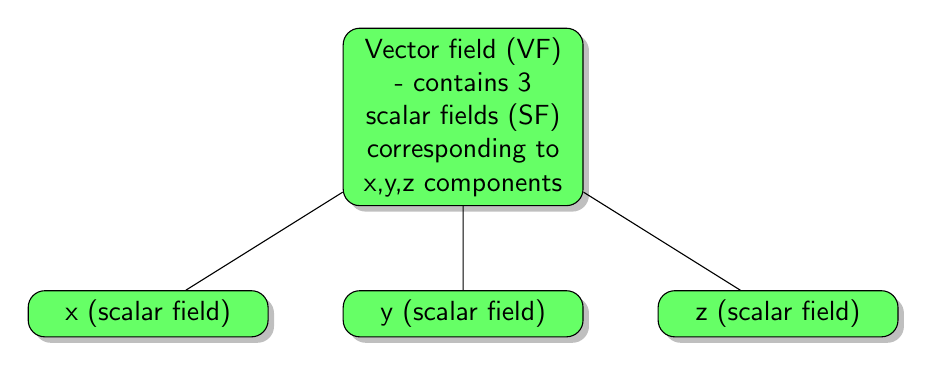
\begin{tikzpicture}[level distance=25mm,level/.style={sibling distance=40mm}]
\node[level 1] {Vector field (VF) - contains 3 scalar fields (SF) corresponding to x,y,z components}
		child { node[level 1] (c1) {x (scalar field)} }
		child { node[level 1] (c1) {y (scalar field)} }
		child { node[level 1] (c1) {z (scalar field)} };
\end{tikzpicture}

\end{document}